\documentclass[a4paper]{article}

\usepackage[fontset=fandol]{ctex}
\usepackage{amsmath, amssymb}
\usepackage{graphicx}
\usepackage[margin=2.35cm]{geometry}
\usepackage[most]{tcolorbox}
\usepackage{etoolbox}
\usepackage{listings}
\usepackage{hyperref}
\usepackage{xurl}
\usepackage{booktabs}
\usepackage{longtable}
\usepackage{tabularx}
\usepackage{array}
\usepackage{subcaption}
\usepackage{float}
\usepackage{enumitem}
\usepackage{tikz}
\usetikzlibrary{arrows.meta, positioning, shapes.geometric}
\IfFileExists{pgfplots.sty}{
    \usepackage{pgfplots}
    \pgfplotsset{compat=1.18}
}{}

\hypersetup{
    colorlinks=true,
    linkcolor=blue!50!black,
    urlcolor=blue!60!black,
    citecolor=blue!50!black
}

\newtcolorbox{findingbox}[1]{
    enhanced,
    colback=green!5!white,
    colframe=green!45!black,
    colbacktitle=green!45!black,
    coltitle=white,
    fonttitle=\bfseries,
    title=#1,
    sharp corners
}

\newtcolorbox{evidencebox}[1]{
    enhanced,
    colback=blue!4!white,
    colframe=blue!65!black,
    colbacktitle=blue!65!black,
    coltitle=white,
    fonttitle=\bfseries,
    title=#1,
    sharp corners
}

\newtcolorbox{riskbox}[1]{
    enhanced,
    colback=red!4!white,
    colframe=red!70!black,
    colbacktitle=red!70!black,
    coltitle=white,
    fonttitle=\bfseries,
    title=#1,
    sharp corners
}

\newtcolorbox{methodbox}[1]{
    enhanced,
    colback=yellow!9!white,
    colframe=yellow!60!black,
    colbacktitle=yellow!60!black,
    coltitle=black,
    fonttitle=\bfseries,
    title=#1,
    sharp corners
}

\lstset{
    language=bash,
    basicstyle=\ttfamily\small,
    keywordstyle=\color{blue},
    stringstyle=\color{red!60!black},
    commentstyle=\color{green!50!black},
    breaklines=true,
    frame=single,
    numbers=left,
    numberstyle=\tiny\color{gray},
    captionpos=b,
    extendedchars=false
}

\newcolumntype{Y}{>{\raggedright\arraybackslash}X}
\setlist[itemize]{leftmargin=1.8em}

\newcommand{\reporttitle}{Lecture2Notes Slide Structure Analysis 深度研究}
\newcommand{\reportsubtitle}{文档、代码、论文与实跑 case 的联合拆解，以及它对现有 video-note pipeline 的可迁移价值}
\newcommand{\reportauthors}{Codex}
\newcommand{\reportdate}{2026-03-26}
\newcommand{\researchquestion}{Lecture2Notes 的 Slide Structure Analysis 到底如何工作？它在真实实跑中的优势和断点是什么？其中哪些思想值得迁移到我们当前的视频笔记可视化链路里？}
\newcommand{\reportscope}{聚焦 SSA 本身及其上下游接口：官方文档、仓库实现、论文描述、与本地实跑 case。默认以英文 slide-heavy 场景评估该模块，再讨论其对中文视频笔记 pipeline 的迁移边界。}
\newcommand{\reportaudience}{正在维护或设计视频讲义 / PDF 生成 pipeline 的工程人员，尤其是关心 slide-heavy 模式优化的人}
\newcommand{\sourcewindow}{外部资料访问与本地实跑均截至 2026-03-26}
\newcommand{\reportcoverpath}{figures/slide3-annotated.png}

\begin{document}

\begin{titlepage}
\centering
{\Large 深度研究报告\par}
\vspace{1.0cm}
{\huge\bfseries \reporttitle\par}
\vspace{0.5cm}
{\Large \reportsubtitle\par}
\vspace{0.9cm}
{\large \reportauthors\par}
\vspace{0.2cm}
{\large \reportdate\par}
\vspace{1.0cm}
\includegraphics[width=0.84\textwidth,height=0.42\textheight,keepaspectratio]{\reportcoverpath}\par
\vfill
\begin{tcolorbox}[width=0.94\textwidth, colback=black!2!white, colframe=black!60, sharp corners]
\textbf{核心问题}：\researchquestion\par
\textbf{研究范围}：\reportscope\par
\textbf{目标读者}：\reportaudience\par
\textbf{证据窗口}：\sourcewindow\par
\end{tcolorbox}
\end{titlepage}

\tableofcontents
\newpage

\section{执行摘要}

\begin{findingbox}{一句话判断}
Lecture2Notes 的 SSA 不是一个“理解整段视频”的模块，而是一个建立在\textbf{已提纯唯一 slide 图像集合}之上的\textbf{OCR 后处理与轻量版式分类器}。它最有价值的思想不是 Tesseract 本身，而是把 slide 转成带有 \texttt{title / bold / normal / footer} 语义的结构化中间层；它最明显的局限，则是对 OCR 噪声、英文词典、硬编码阈值和页面模板非常敏感。
\end{findingbox}

\begin{itemize}
\item 在 Lecture2Notes 的完整链路里，SSA 排在 slide classifier、black border removal / perspective crop、clustering 去重之后。也就是说，它默认输入已经是“最佳 slide 样本”，而不是任意视频帧。
\item SSA 的核心算法非常简单：用 Tesseract 提取词级 OCR 与 bounding box，计算每个词的 stroke width，再按行聚合，用相对均值阈值把每行分类成 \texttt{bold}、\texttt{normal}、\texttt{footer}，并用另一套规则识别第一页第一段是否是 \texttt{title}。
\item 论文和文档都说“Tesseract 输出会被 SymSpell spell check”，但代码实际只对 \texttt{slide-ocr.txt} 这种原始文本做了 spell check；用于下游结构化摘要的 \texttt{slide-ssa.json} 仍保留原始 OCR 错误。
\item 我在当前机器上实际跑了它的 SSA 核心，对一个公开英文 slide deck 的前 8 页做了测试。结果显示：8 页中只有 1 页成功识别出 \texttt{title}；封面页因为上方装饰线被 OCR 成 ``re``，导致标题识别失效；普通 outline 页里的 footer 没被稳定过滤；技术词和数学记号在 SymSpell 后反而被破坏。
\item 因此，SSA \textbf{不适合作为我们 pipeline 的通用主干}，但其“把 slide OCR 提炼为结构化中间表示”的思路非常值得借。对于我们的系统，更合理的路线是：只在 \texttt{slide-heavy / static-outline / screen-demo} 模式下启用一种\textbf{现代化 SSA}，换用更强的 OCR / layout 能力，并把产物写成 \texttt{structured\_slide.json} 或 \texttt{layout\_transcript.json}。
\end{itemize}

\begin{riskbox}{最重要的迁移结论}
如果直接把 Lecture2Notes 的 Tesseract + stroke-width heuristics 原样搬进来，在中文、多公式、UI、白板、评论视频里会迅速失效。应该迁移的是中间层思想，而不是旧 OCR 栈和硬编码阈值。
\end{riskbox}

\section{研究范围与方法}

\subsection{本报告回答什么问题}

本报告聚焦四个问题：

\begin{enumerate}
\item Lecture2Notes 的 SSA 在整个系统中扮演什么角色？
\item 它的算法、代码路径、输入输出结构到底是什么？
\item 在当前机器和一个真实 case 上跑起来之后，它表现如何，暴露出哪些断点？
\item 它能否优化我们当前的 video-note pipeline，如果能，应该借什么、不借什么？
\end{enumerate}

\subsection{证据来源}

\begin{methodbox}{证据组成}
\begin{itemize}
\item 官方资料：Lecture2Notes 文档、README、论文 PDF。
\item 源码：本地 clone 的 \texttt{slide\_structure\_analysis.py}、\texttt{spell\_check.py}、\texttt{summarizer\_class.py}、\texttt{summarization\_approaches.py}。
\item 实跑：选取一个公开英文 slide deck，将前 8 页导成 PNG，直接调用 SSA 核心进行分析。
\item 环境审查：检查原项目 \texttt{environment.yml} 与当前机器的二进制 / Python 包差异，定位兼容性断点。
\end{itemize}
\end{methodbox}

\subsection{为什么 case 选英文 slide，而不是我们的中文视频}

这是一个刻意选择。原因有三点：

\begin{itemize}
\item Lecture2Notes 的 SSA 文档、SymSpell 词典和论文实验默认都是英文 slide-heavy 语境；
\item 当前机器默认没有英文 \texttt{eng} Tesseract 语言包，我是手动补的；如果再直接测中文，结果会被语言包问题污染；
\item 我们此处要回答的是“模块原理与迁移价值”，所以应先在它最擅长的语境里评估，再讨论迁移边界。
\end{itemize}

\section{Lecture2Notes 全链路里，SSA 在哪里}

\subsection{SSA 不是前置定位器，而是后置结构化器}

官方文档和 README 都把端到端流程描述为：

\begin{enumerate}
\item 抽帧
\item slide classifier 区分 \texttt{slide} 与 \texttt{presenter\_slide}
\item black border removal / perspective crop
\item clustering 去重并挑出最佳 slide 样本
\item 对唯一 slide 样本运行 SSA
\item figure detection
\item ASR / transcript
\item 组合 slide transcript 与音频 transcript，再做 summarization
\end{enumerate}

这意味着 SSA 的前提非常强：它不是拿来解决“视频里哪里有关键图”的，而是拿来解决“我已经有一组不错的 slide 图片了，现在如何把它们转成结构化文本”。

\begin{figure}[H]
\centering
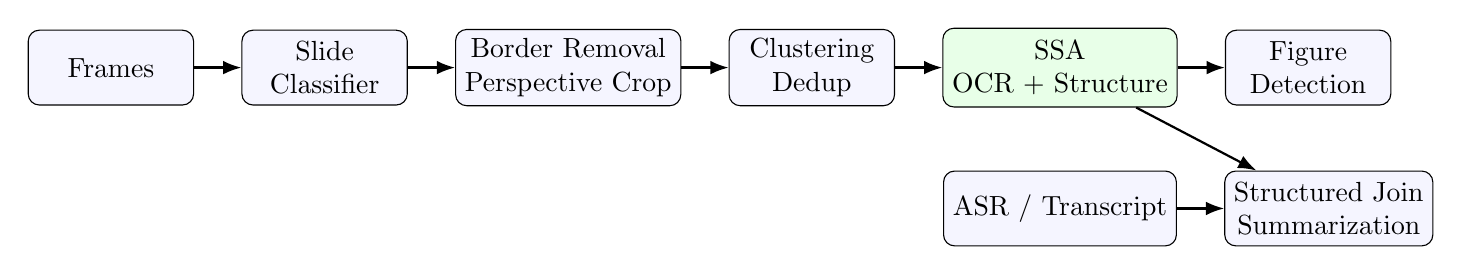
\begin{tikzpicture}[
    node distance=0.8cm and 0.6cm,
    box/.style={draw, rounded corners, align=center, minimum height=0.95cm, minimum width=2.1cm, fill=blue!4},
    ssa/.style={draw, rounded corners, align=center, minimum height=1.0cm, minimum width=2.2cm, fill=green!9},
    arrow/.style={-Latex, thick}
]
\node[box] (frames) {Frames};
\node[box, right=of frames] (classifier) {Slide\\Classifier};
\node[box, right=of classifier] (crop) {Border Removal\\Perspective Crop};
\node[box, right=of crop] (cluster) {Clustering\\Dedup};
\node[ssa, right=of cluster] (ssa) {SSA\\OCR + Structure};
\node[box, right=of ssa] (figure) {Figure\\Detection};
\node[box, below=of ssa] (transcript) {ASR / Transcript};
\node[box, right=of transcript] (summary) {Structured Join\\Summarization};

\draw[arrow] (frames) -- (classifier);
\draw[arrow] (classifier) -- (crop);
\draw[arrow] (crop) -- (cluster);
\draw[arrow] (cluster) -- (ssa);
\draw[arrow] (ssa) -- (figure);
\draw[arrow] (ssa) -- (summary);
\draw[arrow] (transcript) -- (summary);
\end{tikzpicture}
\caption{Lecture2Notes 中 SSA 的位置：它服务于“已去重 slide 集合”的结构化，而不是服务于视频关键帧搜索}
\end{figure}

\subsection{这件事对我们为什么重要}

它直接决定了是否值得迁移。我们当前 pipeline 最大的痛点之一，是还没稳定产出“最终可解释的 figure plan 与 frame manifest”。Lecture2Notes 的 SSA 并不能帮我们解决“如何从视频定位图”，但它能启发我们在 slide-heavy 模式下增加一层：

\begin{center}
候选 slide 图像 $\rightarrow$ 结构化 slide transcript
\end{center}

这对章节标题、强调行、正文结构、footer 过滤都很有帮助。

\section{SSA 的工作原理}

\subsection{输入、输出与产物}

代码层面，SSA 的主入口是：

\begin{itemize}
\item \texttt{analyze\_structure(image, ...)}
\item \texttt{all\_in\_folder(path, ...)}
\item \texttt{write\_to\_file(raw\_texts, json\_texts, ...)}
\end{itemize}

其中：

\begin{itemize}
\item 输入是一张 slide 图像，或一个装有 slide 图像的文件夹；
\item 输出有两类：
  一类是原始 OCR 合并文本；
  一类是结构化 JSON，其中按行保存文本及其类别；
\item 如果在完整 Summarizer 流程里运行，还会额外写出：
  \texttt{slide-ocr.txt} 和 \texttt{slide-ssa.json}
\end{itemize}

\subsection{OCR 层：词级别 Tesseract，保留位置与层级元数据}

SSA 首先调用 Tesseract 的 \texttt{image\_to\_data}，拿到词级别输出。与纯 \texttt{image\_to\_string} 不同，这里保留了：

\begin{itemize}
\item \texttt{block\_num}
\item \texttt{par\_num}
\item \texttt{line\_num}
\item \texttt{word\_num}
\item 每个词的 \texttt{left, top, width, height}
\end{itemize}

这个设计很关键。因为 SSA 后面并不是直接按词输出，而是要恢复“哪一堆词属于同一行、同一段”，再对行级对象做分类。

\subsection{stroke width：它不是 OCR 置信度，而是字体粗细的近似代理}

SSA 最独特的地方，是它没有只依赖 bounding box 高度，而是额外计算了每个词图像块的 stroke width。其流程可写成：

$$
\text{SW}(w) = \operatorname{mean}\left(\operatorname{PeakLocalMax}\left(\operatorname{DT}\left(\operatorname{OtsuBin}(w)\right)\right)\right)
$$

\begin{itemize}
\item $w$：某个词的图像块
\item $\operatorname{OtsuBin}$：Otsu 阈值分割，并在代码中做反色二值化
\item $\operatorname{DT}$：距离变换
\item $\operatorname{PeakLocalMax}$：对距离图取局部峰值
\item $\text{SW}(w)$：这些峰值的平均值，作为词的笔画粗细近似
\end{itemize}

直觉上，标题和粗体文本通常拥有更大的 stroke width，而页脚和小字则更小。

\subsection{从词到行：通过全局 line 编号恢复可分类单元}

SSA 会扫描 OCR DataFrame，并用一个简单规则重建 \texttt{global\_line\_num}：

\begin{itemize}
\item 每当 \texttt{word\_num == 1}，就认为开启了一条新行；
\item 然后对同一 \texttt{global\_line\_num} 的词做聚合；
\item 文本列做字符串拼接，其余数值列求均值。
\end{itemize}

因此，真正被分类的对象不是词，也不是段落，而是\textbf{行}。

\subsection{行分类：一个非常硬的阈值逻辑}

在代码里，行分类分为四类：

\begin{itemize}
\item \texttt{2}: title
\item \texttt{1}: subtitle / bold
\item \texttt{0}: normal
\item \texttt{-1}: small / footer
\end{itemize}

对非 title 行，核心分类规则可以写成：

$$
\text{cat}(l)=
\begin{cases}
1, & s_l > \bar{s}(1+\gamma) \ \lor\  h_l > \bar{h}(1+\beta) \\
-1, & s_l < \bar{s}(1-\gamma) \ \land\ h_l < \bar{h}(1-\beta) \\
0, & \text{otherwise}
\end{cases}
$$

\begin{itemize}
\item $l$：某一文本行
\item $s_l$：该行平均 stroke width
\item $h_l$：该行平均 bounding box height
\item $\bar{s}$：整页词的平均 stroke width
\item $\bar{h}$：整页词的平均高度
\item $\gamma$：stroke width 阈值，默认 $0.1$
\item $\beta$：height 阈值，默认 $0.2$
\end{itemize}

这个规则有两个鲜明特征：

\begin{itemize}
\item 它对 \texttt{bold} 很宽松，只要 “stroke 宽” 或 “字高高” 任一成立即可；
\item 它对 \texttt{footer} 很严格，必须两个条件同时偏小。
\end{itemize}

这解释了为什么它宁愿把一些正文误判成 bold，也不愿轻易把正文误删成 footer。

\subsection{title detection：完全依赖“第一页第一段”的几何假设}

title detection 不是机器学习，而是另一套规则：

\begin{enumerate}
\item 必须是第一 block 的第一 paragraph；
\item 其平均 \texttt{top} 在页面上三分之一；
\item 其平均 \texttt{left} 小于页面宽度的 $77\%$；
\item 字符数超过 3；
\item 平均 stroke width 高于全页均值加一个标准差；
\item 平均字高高于全页平均字高。
\end{enumerate}

如果整页只有一个 block / paragraph，则第 5 和第 6 条被关闭，以免“整页平均”退化成标题本身。

\begin{findingbox}{SSA 的本质}
SSA 不是一个学习型版面分析模型，而是一套“词级 OCR + 词图像 stroke width + 行级阈值分类 + 第一段标题规则”的启发式系统。
\end{findingbox}

\subsection{spell check：论文说得很强，代码落点却很弱}

官方文档和论文都写了 “All Tesseract outputs are spell checked with SymSpell”。但实际代码路径是：

\begin{itemize}
\item \texttt{slide\_structure\_analysis.all\_in\_folder()} 产出 \texttt{raw\_texts} 和 \texttt{json\_texts}
\item \texttt{summarizer\_class.step\_slide\_structure\_analysis()} 只对 \texttt{raw\_texts} 调用 \texttt{SpellChecker.check\_all()}
\item 随后把\textbf{已 spell-check 的 raw text}与\textbf{未 spell-check 的 json\_texts}一起写盘
\end{itemize}

这意味着：

\begin{itemize}
\item \texttt{slide-ocr.txt} 可能是拼写纠正后的；
\item 但 \texttt{slide-ssa.json} 里保存的结构化文本，仍然保留原始 OCR 错误；
\item 下游 \texttt{structured\_joined\_sum()} 读取的是 SSA JSON，所以它实际上消费的是\textbf{未纠正 OCR}。
\end{itemize}

\section{源码层面的关键观察}

\subsection{它依赖的前提，比文档看起来更强}

从 \texttt{end\_to\_end/general.rst} 和 \texttt{summarizer\_class.py} 可以看到，SSA 默认处理的是聚类后最佳 slide 样本目录 \texttt{best\_samples\_dir}。因此它对输入假设非常强：

\begin{itemize}
\item 图像已被裁成只含 slide 主体；
\item 重复页基本去掉；
\item 排序和 frame number 语义稳定；
\item 语言基本是英文；
\item 模板接近传统课堂 slides。
\end{itemize}

\subsection{它对现代环境并不稳，需要兼容修正}

在当前机器上，我为了跑通 SSA 做了两个极小兼容补丁：

\begin{enumerate}
\item \texttt{slide\_structure\_analysis.py}：
  为空的 stroke width 峰值返回 0，并把 \texttt{grouped.mean()} 改成 \texttt{grouped.mean(numeric\_only=True)}，否则新版 pandas 会报 \texttt{dtype 'str' does not support operation 'mean'}。
\item \texttt{spell\_check.py}：
  不再使用老式的 \texttt{pkg\_resources.resource\_filename}，而是直接从 \texttt{symspellpy} 包目录定位资源文件。
\end{enumerate}

这两个问题说明：\textbf{SSA 的思想仍可用，但原仓库并不是“拿来即跑”的现代可维护组件。}

\subsection{原项目环境相当旧}

原始 \texttt{environment.yml} 还带着：

\begin{itemize}
\item 旧版 PyTorch / TensorFlow
\item conda 环境假设
\item Vosk / DeepSpeech / youtube\_dl / pytorch\_lightning 老组合
\item 默认强依赖英语 NLP 生态
\end{itemize}

这对研究复现没问题，但对直接抽取 SSA 作为一个现代微模块不友好。

\section{实跑 case}

\subsection{Case 选择}

本次 case 选择公开 slide deck：

\begin{itemize}
\item 来源：\url{https://seuml.github.io/ml-spring-2024/assets/slides/lecture2.pdf}
\item 标题：\texttt{Lecture 2: Linear Regression}
\item 页数：70 页
\item 本次只取前 8 页，模拟“已去重后的最佳 slide 样本”
\end{itemize}

\subsection{运行设置}

\begin{itemize}
\item 本地 clone commit：\texttt{10210930ac4c3ffe3de7de0a36b74514122ff445}
\item Python：系统 \texttt{Python 3.14.3}，新建最小 venv
\item OCR：系统 \texttt{tesseract}，额外下载 \texttt{eng.traineddata}
\item 只安装 SSA 所需最小依赖：\texttt{numpy, pandas, pytesseract, scikit-image, opencv-python-headless, tqdm, pillow, symspellpy}
\end{itemize}

\begin{lstlisting}[caption={本次 case 的最小运行步骤}]
python3 -m venv artifacts/venv
source artifacts/venv/bin/activate
pip install numpy pandas pytesseract scikit-image \
  opencv-python-headless tqdm pillow symspellpy

curl -L https://raw.githubusercontent.com/tesseract-ocr/tessdata_fast/main/eng.traineddata \
  -o artifacts/tessdata/eng.traineddata

pdftoppm -f 1 -l 8 -png case/input_pdf/lecture2.pdf case/slides/tmp
# 重命名为 slide_0001.png ... slide_0008.png

TESSDATA_PREFIX=artifacts/tessdata \
PYTHONPATH=artifacts/lecture2notes-repo \
python -c 'from lecture2notes.end_to_end import slide_structure_analysis; ...'
\end{lstlisting}

\subsection{Case 总体结果}

\begin{table}[H]
\centering
\caption{8 页 case 的总体统计}
\begin{tabularx}{\textwidth}{p{3.2cm}Yp{2.4cm}}
\toprule
指标 & 含义 & 结果 \\
\midrule
输入页数 & 抽取并送入 SSA 的 slide 数 & 8 \\
平均每页行数 & \texttt{slide-ssa.json} 中每页保留下来的行数 & 8.62 \\
category=2 & title 行数量 & 1 \\
category=1 & bold / subtitle 行数量 & 32 \\
category=0 & normal 行数量 & 28 \\
category=-1 & footer / small 行数量 & 8 \\
spell-check 影响 & 对 \texttt{slide-ocr.txt} 进行 SymSpell 修正 & 有，但会损伤技术词 \\
\bottomrule
\end{tabularx}
\end{table}

\subsection{三个最关键的页面观察}

\subsubsection{封面页：边框被 OCR 成伪文本，导致标题识别失败}

\begin{figure}[H]
\centering
\begin{subfigure}[t]{0.48\textwidth}
\centering
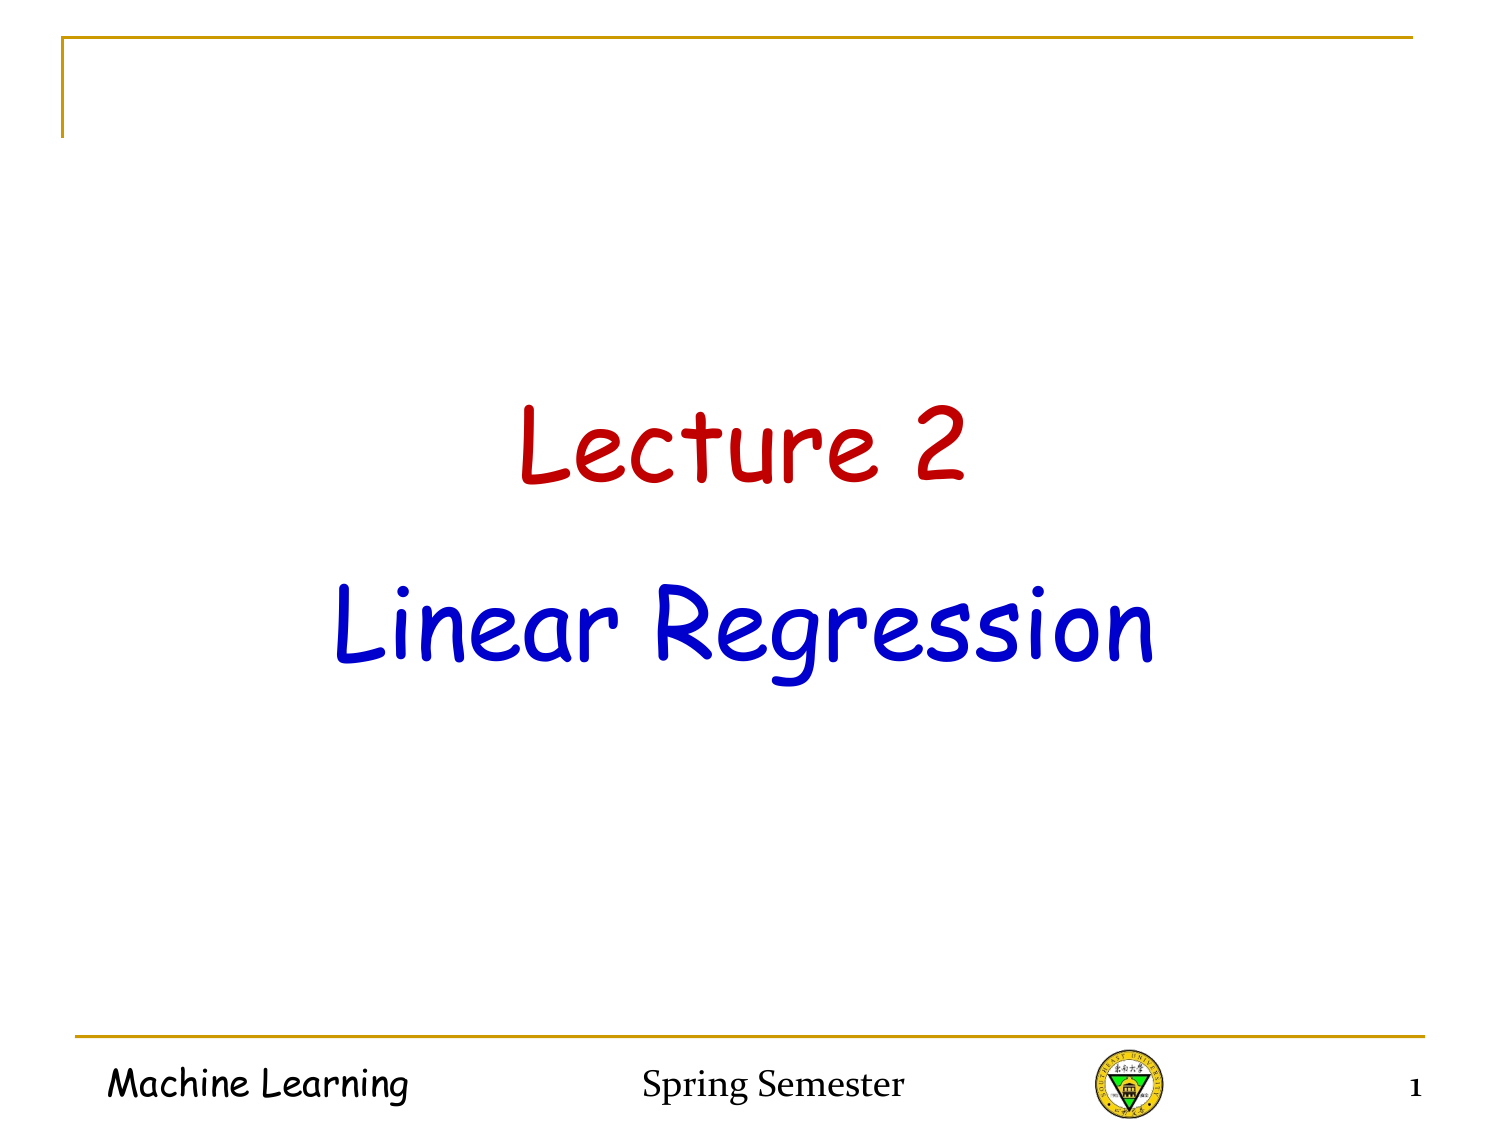
\includegraphics[width=\textwidth]{figures/slide1-original.png}
\caption{原始 slide}
\end{subfigure}
\hfill
\begin{subfigure}[t]{0.48\textwidth}
\centering
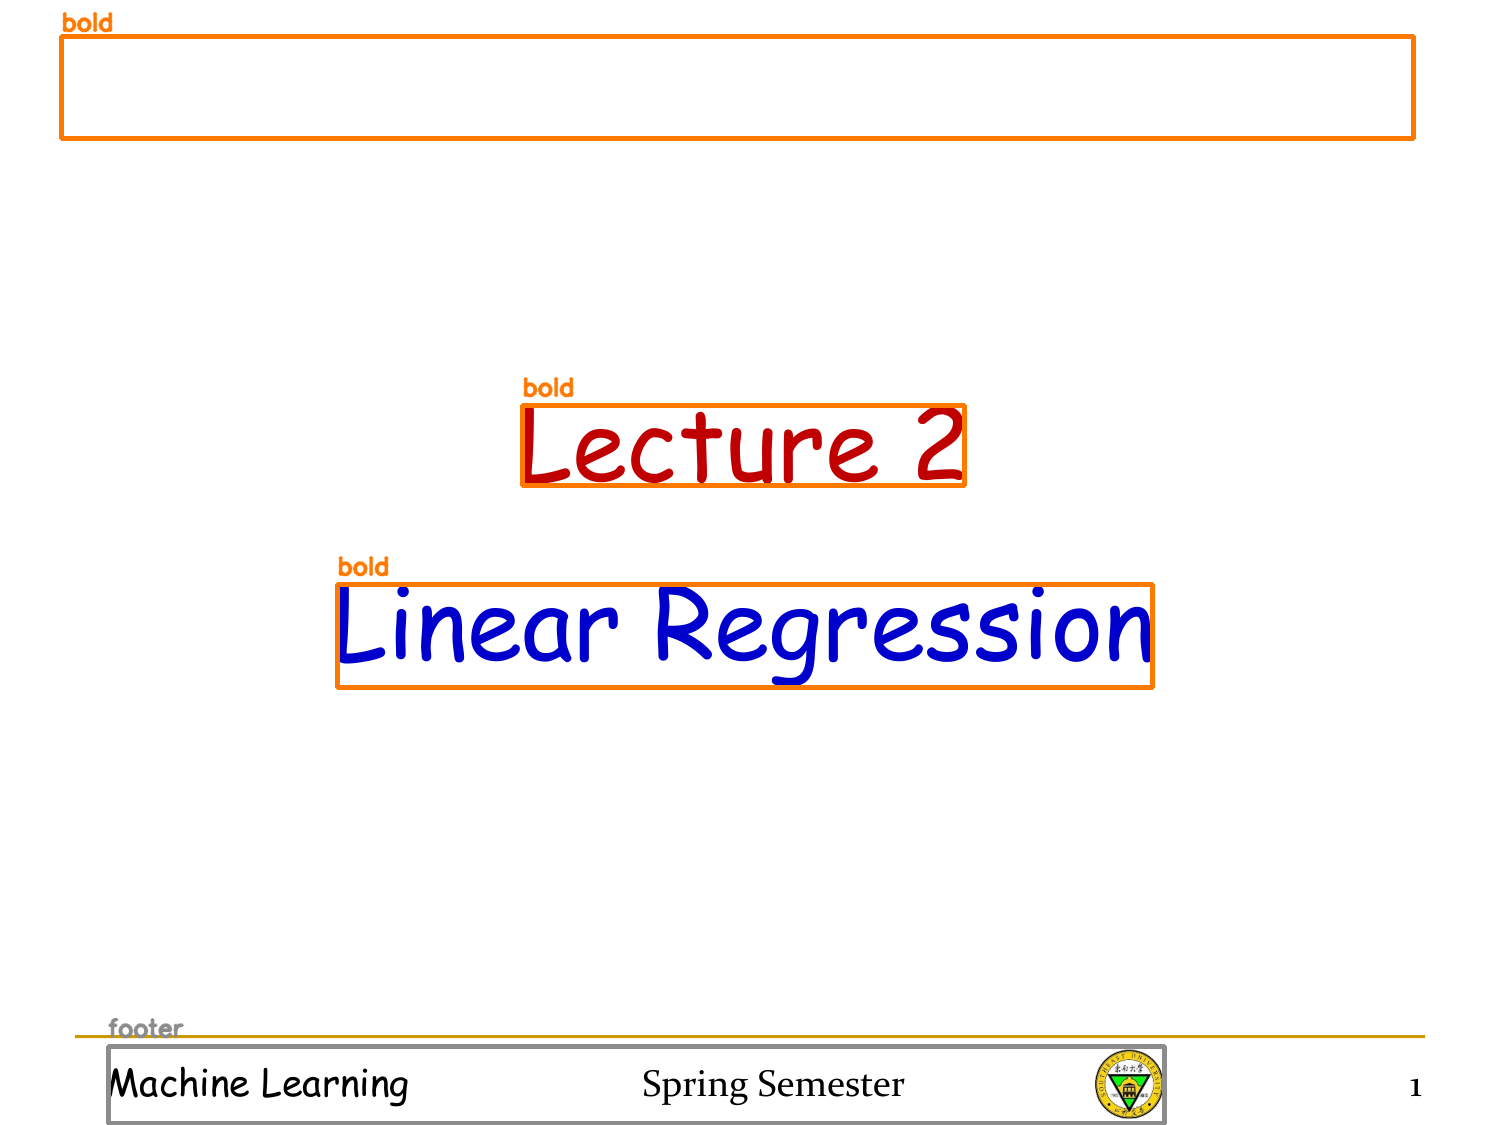
\includegraphics[width=\textwidth]{figures/slide1-annotated.png}
\caption{SSA 行分类结果}
\end{subfigure}
\caption{封面页的顶部装饰线被 OCR 成一条伪文本行 ``re``，因此第一 block 不再是实际标题，导致 title detection 失效}
\end{figure}

调试结果表明，Slide 1 的第一 block 文本是 ``re``，字符数只有 2，不满足 title check 的字符门槛，因此真正的 ``Lecture 2`` 和 ``Linear Regression`` 都只被判成 \texttt{bold}，最终 structured output 的标题退化成默认值 \texttt{Slide 1}。

\subsubsection{普通 outline 页：大纲项被很好区分成强调与正文，但标题没有被识别为 title}

\begin{figure}[H]
\centering
\begin{subfigure}[t]{0.48\textwidth}
\centering
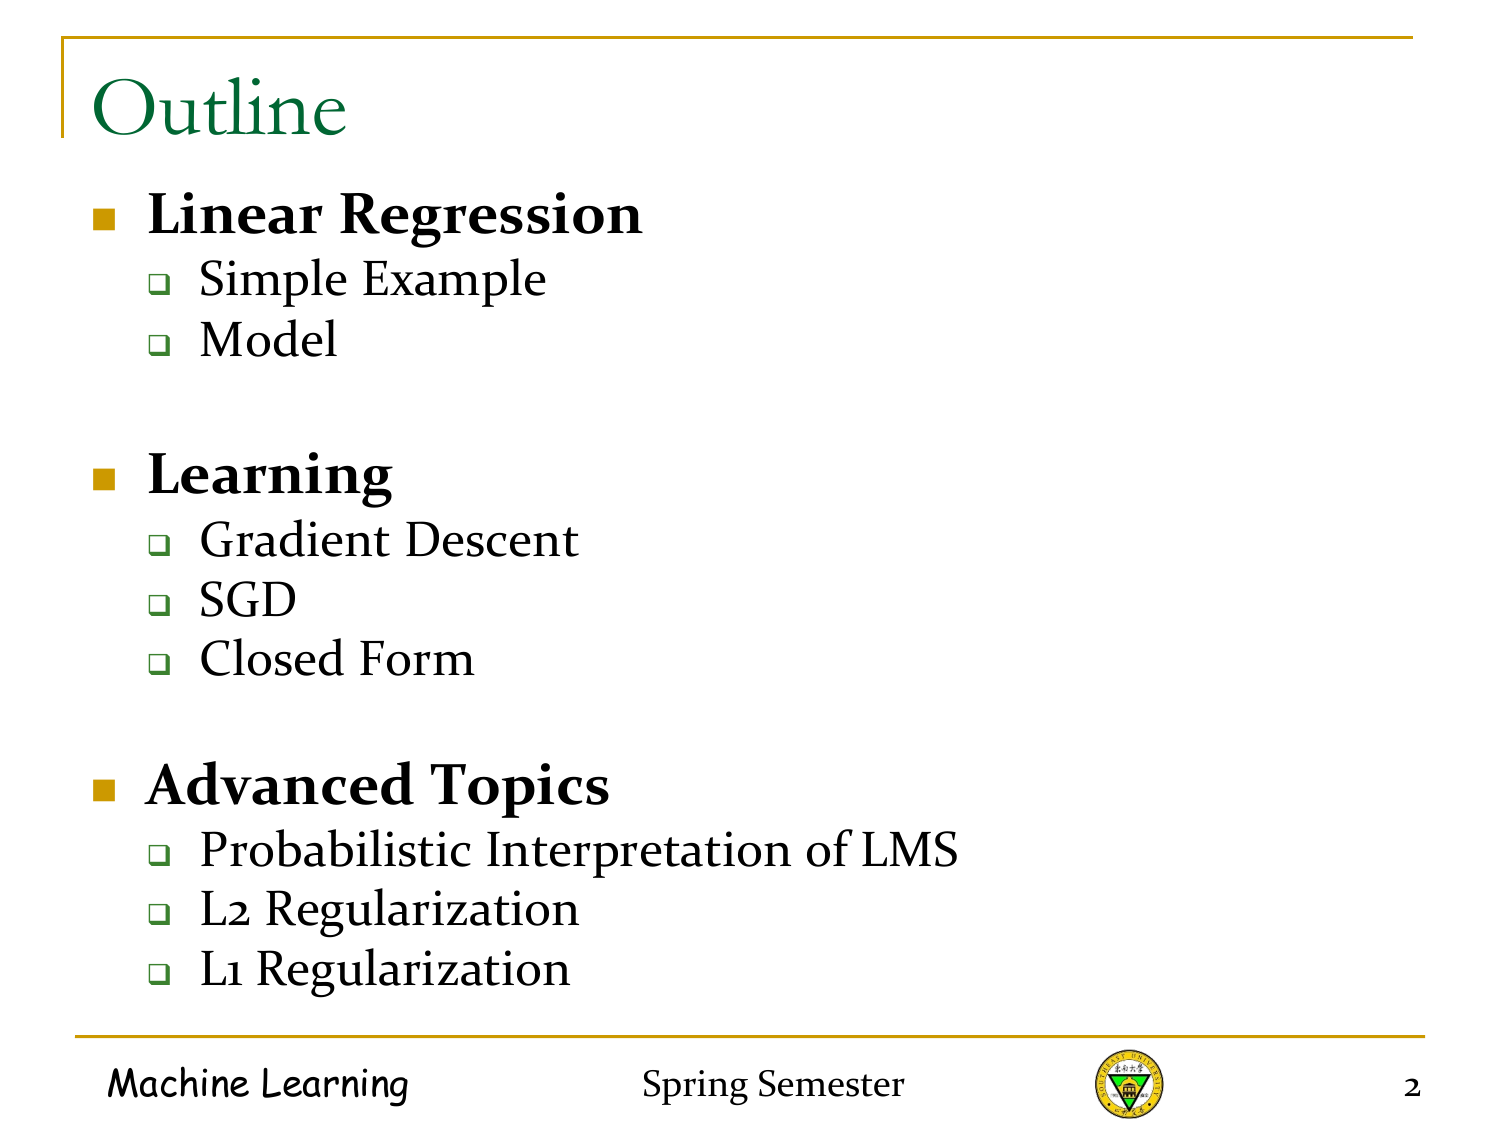
\includegraphics[width=\textwidth]{figures/slide2-original.png}
\caption{原始 outline 页}
\end{subfigure}
\hfill
\begin{subfigure}[t]{0.48\textwidth}
\centering
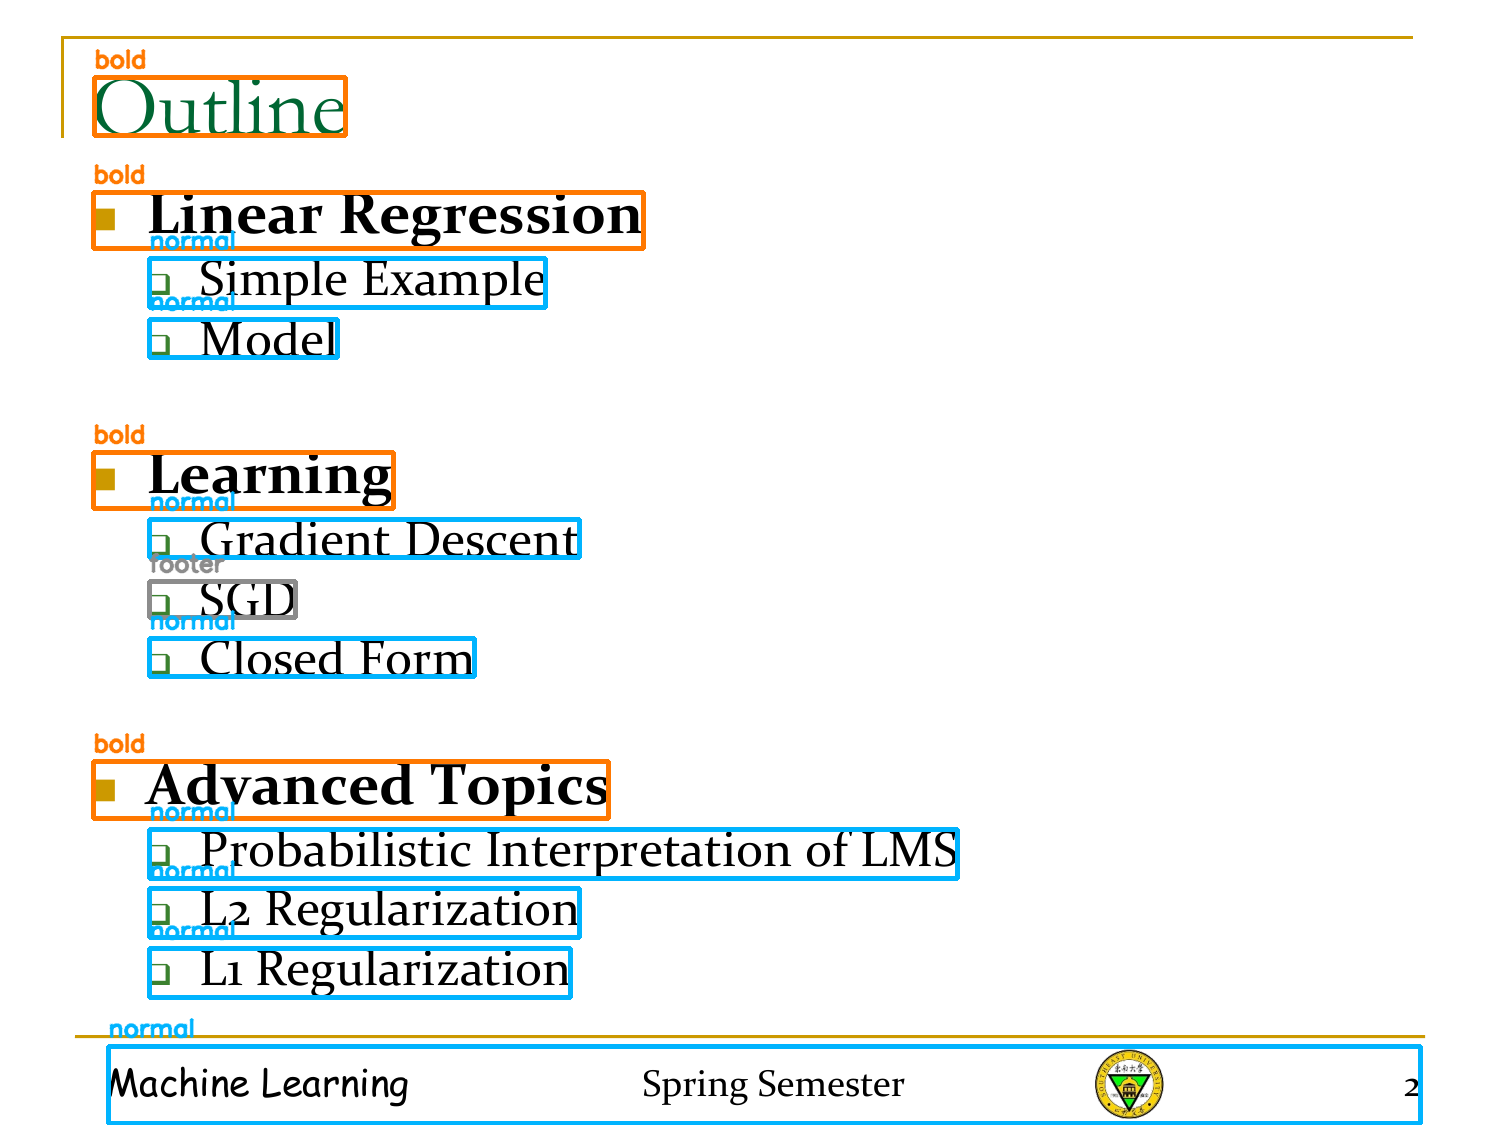
\includegraphics[width=\textwidth]{figures/slide2-annotated.png}
\caption{SSA 结果}
\end{subfigure}
\caption{Slide 2 说明了 SSA 的优点与缺点并存：大纲级别能大体分出来，但页标题 `Outline` 仍未被提升为 title，页脚也没有被完全过滤}
\end{figure}

对 Slide 2，SSA 的优点是明显的：

\begin{itemize}
\item \texttt{Linear Regression}、\texttt{Learning}、\texttt{Advanced Topics} 这类大纲层级被判成 \texttt{bold}
\item 子项大多被判成 \texttt{normal}
\end{itemize}

但它的缺点也同样明显：

\begin{itemize}
\item 顶部标题 \texttt{Outline} 因 stroke width 不够大，没有进入 \texttt{title}
\item 页脚 \texttt{Machine Learning Spring Semester ...} 被保留成 \texttt{normal}
\item \texttt{SGD} 被误判成 \texttt{footer}
\end{itemize}

\subsubsection{公式页：标题终于识别成功，但正文中很多数学行被抬升成 bold}

\begin{figure}[H]
\centering
\begin{subfigure}[t]{0.48\textwidth}
\centering
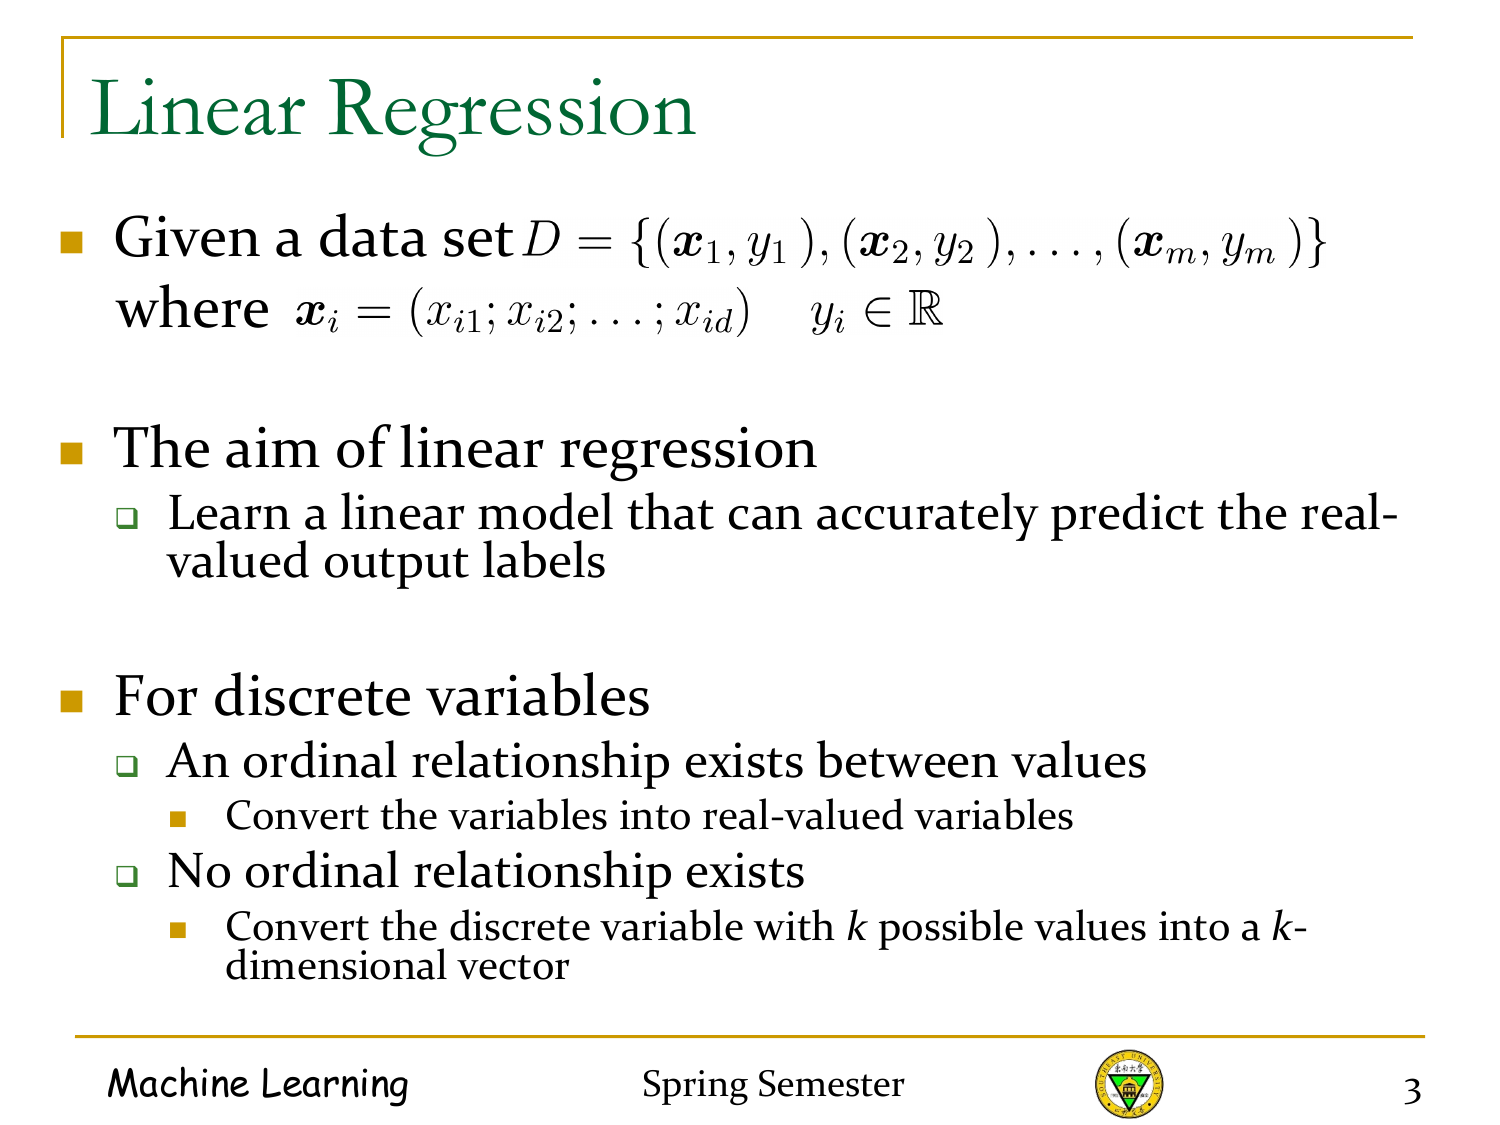
\includegraphics[width=\textwidth]{figures/slide3-original.png}
\caption{原始 slide}
\end{subfigure}
\hfill
\begin{subfigure}[t]{0.48\textwidth}
\centering
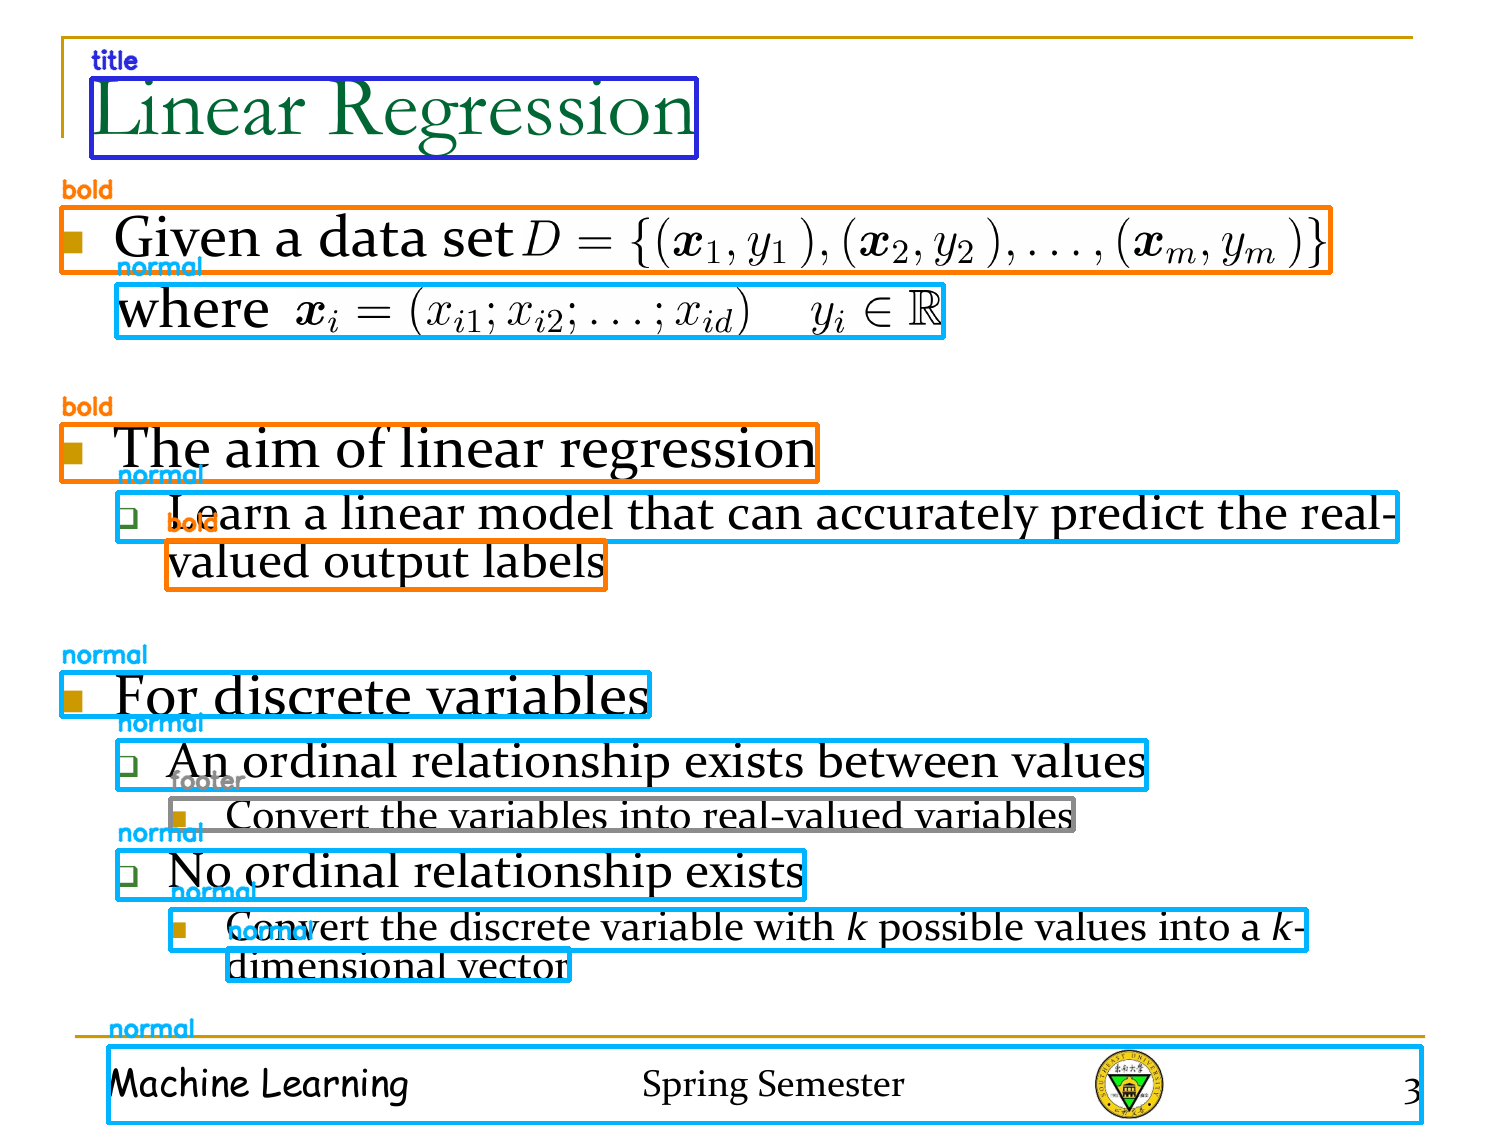
\includegraphics[width=\textwidth]{figures/slide3-annotated.png}
\caption{SSA 结果}
\end{subfigure}
\caption{Slide 3 是 8 页里唯一成功 title detection 的页面，但也显示了“高字高 / 高 stroke 容易把正文推成 bold”的副作用}
\end{figure}

这一页里，\texttt{Linear Regression} 正确被识别为 \texttt{title}。但正文中的公式和章节句首也经常因为行高更大而被判成 \texttt{bold}。这对“做 outline”未必是坏事，但对“忠实恢复原 slide 结构”就已经偏粗糙了。

\subsection{结构化输出的 downstream 影响}

把 \texttt{slide-ssa.json} 按 \texttt{structured\_joined\_sum()} 的逻辑消费后，前 8 页的 slide 标题大致会变成：

\begin{table}[H]
\centering
\caption{前 8 页 slide 的标题产出结果}
\begin{tabularx}{\textwidth}{p{1.4cm}p{3.1cm}Y}
\toprule
页码 & 实际视觉标题 & 下游生成标题 \\
\midrule
1 & Lecture 2 / Linear Regression & Slide 1 \\
2 & Outline & Slide 2 \\
3 & Linear Regression & Linear Regression \\
4 & Linear Regression & Slide 4 \\
5 & Linear Regression example & Slide 5 \\
6 & Linear Regression example & Slide 6 \\
7 & Linear Regression example & Slide 7 \\
8 & Linear Regression & Slide 8 \\
\bottomrule
\end{tabularx}
\end{table}

也就是说，在本次 case 里，\textbf{8 页只有 1 页能够把视觉标题真正下沉为结构化标题键}。这对后续生成“按 slide 标题组织的结构化讲义”显然是不够稳的。

\subsection{spell-check 的真实影响}

\begin{evidencebox}{一次很有代表性的 before / after}
未 spell-check：

\small
\texttt{... Probabilistic Interpretation of LMS ... L2 Regularization ... Li Regularization ...}
\normalsize

经 SymSpell 后：

\small
\texttt{... probabilistic interpretation of los ... la regularization ... i regularization ...}
\normalsize
\end{evidencebox}

这说明 SymSpell 的确能修一些普通英语词，但对技术缩写、数学记号、层级标记、课程模板文本并不友好。对我们今天的视频笔记场景，尤其是中文、公式、代码、界面控件文本，这一步基本不能原样照搬。

\section{Lecture2Notes SSA 值得借什么，不值得借什么}

\subsection{最值得借的，不是 Tesseract，而是“结构化 slide transcript”}

Lecture2Notes 给我们的最大启发不是 OCR 引擎，而是 artifact 设计：

\begin{itemize}
\item 不要把 slide OCR 只当成一坨纯文本；
\item 应该把它变成“按行组织的结构化表示”，并保留语义类别；
\item 这样下游才能做：
  章节标题抽取、
  强调行提炼、
  footer 过滤、
  transcript 与 slide 的结构对齐。
\end{itemize}

这正对应我们当前 pipeline 的一个空白：字幕之后还缺一层能够把“图像里的文字结构”稳定描述出来的中间层。

\subsection{最不该借的，是旧 OCR 栈与硬编码阈值}

直接照搬 Lecture2Notes SSA 会遇到这些问题：

\begin{itemize}
\item 默认假设英语，且依赖英语词典 spell check；
\item 依赖 Tesseract block / paragraph 的稳定性，而现代 slides 上 logo、装饰线、页码、导航条都可能打乱第一 block；
\item 只用 stroke width 与字高做判断，无法处理 code block、公式、UI、表格、混合语言；
\item footer 规则过死，必须两个尺度都偏小；
\item 对 progressive reveal、screen-demo、白板视频几乎没有直接帮助。
\end{itemize}

\subsection{对我们 pipeline 的可迁移价值}

我建议把它拆成“概念层”和“实现层”来判断。

\subsubsection{概念层：值得迁移}

\begin{itemize}
\item 在 \texttt{slide-heavy / static-outline / screen-demo} 模式里，加入一层 \texttt{structured\_slide.json}
\item 该 JSON 至少记录：
  标题候选、
  强调行、
  正文行、
  footer / boilerplate、
  以及它们对应的图像区域
\item 下游用它来：
  辅助章节命名、
  生成 callout、
  过滤 footer、
  对 PDF 正文做逻辑压缩
\end{itemize}

\subsubsection{实现层：需要现代化重写}

\begin{table}[H]
\centering
\caption{Lecture2Notes SSA 与我们更合理实现的对照}
\begin{tabularx}{\textwidth}{p{3.1cm}p{4.0cm}Y}
\toprule
环节 & Lecture2Notes 做法 & 更适合我们的做法 \\
\midrule
OCR & Tesseract 英文 OCR & PaddleOCR / docTR / 更强多语言 OCR \\
文本组织 & 词级 OCR 后按行聚合 & 保留行和区域，两层结构都留 \\
类别判定 & stroke width + height heuristics & 几何特征 + OCR 置信度 + layout analysis + 可选 VLM 纠偏 \\
title detection & 第一 block / 第一 paragraph 规则 & 多候选标题区域 + 模式化校验，不只盯第一段 \\
spell check & 英文 SymSpell & 按语言与模式选择，技术词不要默认纠正 \\
适用模式 & 传统英文 slide-heavy lecture & 只在 slide-heavy / static-outline / screen-demo 中按需启用 \\
\bottomrule
\end{tabularx}
\end{table}

\subsection{它具体能优化我们哪个部分}

如果只谈 ROI，我认为它对我们现有系统最有帮助的是这三个点：

\begin{enumerate}
\item \textbf{章节结构提炼}
  
  对 slide-heavy 视频，slide 标题和大纲项常常比 transcript 更稳定。一个现代化 SSA 能帮助 outline 阶段更快得到章标题与小节骨架。

\item \textbf{图文规划}
  
  如果知道某页 slide 的“主标题、强调项、正文、页脚”分布，agent 在决定“放整页图还是只裁一块”时会更有依据。

\item \textbf{PDF 正文压缩}
  
  对 \texttt{static-outline} 和某些 screen-demo，结构化 slide transcript 能帮我们在 PDF 里更自然地用项目符号、强调块和表格重写，而不是依赖长段 OCR 原文。
\end{enumerate}

\subsection{它明确帮不了我们的部分}

\begin{itemize}
\item 不能替代关键帧搜索：它不处理“从视频里哪里找图”
\item 不能处理白板累积：它没有 progressive reveal 最终态搜索能力
\item 不能处理 commentary：这类视频的高价值信息不在 slide 结构里
\item 不能直接解决中文 / 公式 / UI 多样性：旧 OCR 与英文词典都不适配
\end{itemize}

\begin{findingbox}{对我们最实际的建议}
不要引入原版 Lecture2Notes SSA；应该引入一层\textbf{SSA-like artifact}。也就是在 slide-heavy 模式下，新增一个现代化的结构化版面转写模块，把候选 slide 图像变成可被大纲生成与 PDF 写作消费的中间表示。
\end{findingbox}

\section{建议的迁移方案}

\subsection{P0：先做轻量版结构化 slide transcript}

\begin{itemize}
\item 只在 \texttt{slide-heavy / static-outline} 模式启用
\item 对最终候选 slide 图运行 OCR
\item 不做复杂分类，只先做三类：
  \texttt{title-candidate}、
  \texttt{body}、
  \texttt{footer-candidate}
\item 产出 \texttt{structured\_slide.json}
\end{itemize}

\subsection{P1：接入更强 layout}

\begin{itemize}
\item 用 PaddleOCR layout analysis 或类似模块代替手工几何阈值
\item 保留文本块区域，辅助 crop 与 PDF 图注生成
\item 在公式页、表格页、UI 页加专门 probe
\end{itemize}

\subsection{P2：让 agent / VLM 做纠偏，而不是做主干}

\begin{itemize}
\item 让确定性 OCR / layout 先产出候选结构
\item 再让 VLM 判断哪个标题候选最像本页主题
\item VLM 只做纠偏和排序，不直接取代底层 artifact
\end{itemize}

\section{结论与后续问题}

\subsection{已经有充分证据支持的结论}

\begin{itemize}
\item Lecture2Notes SSA 是一个后置结构化模块，不是视频定位模块。
\item 它的核心是启发式：OCR + stroke width + height + 几何标题规则。
\item 它最有价值的是“把 slide 文本结构化”，而不是具体的 OCR 栈。
\item 在真实英文 case 上，它连 title detection 都不够稳；普通现代 slides 上，装饰线和页脚就足以破坏规则。
\item 论文 / 文档与代码之间存在一处重要落差：spell-check 并没有真正进入 SSA JSON。
\end{itemize}

\subsection{大概率正确但仍值得继续验证的推断}

\begin{itemize}
\item 如果换成更强多语言 OCR + layout analysis，这种 “SSA-like artifact” 对我们的 slide-heavy 视频会非常有帮助。
\item 对中文投资视频、读书视频、软件演示视频，结构化版面转写比纯 OCR 原文更可能提升 PDF 逻辑质量。
\item 对 commentary 和 board-heavy 视频，这层的收益会明显下降，应通过 mode routing 控制。
\end{itemize}

\subsection{下一步最值得做的两件事}

\begin{enumerate}
\item 在我们现有 pipeline 里设计一个 \texttt{structured\_slide.json}，先只面向 \texttt{slide-heavy / static-outline} 模式。
\item 用现代 OCR / layout 工具做一个小实验，对比 “纯 OCR 原文” 和 “结构化 slide transcript” 对 PDF 大纲质量、footer 过滤和标题抽取的改善幅度。
\end{enumerate}

\appendix

\section{来源清单}
\small
\begin{longtable}{p{1.4cm}p{1.7cm}p{4.2cm}p{6.8cm}}
\toprule
Source ID & 模态 & 标题 / 标签 & 链接或路径 \\
\midrule
\endfirsthead
\toprule
Source ID & 模态 & 标题 / 标签 & 链接或路径 \\
\midrule
\endhead
W1 & Web & Lecture2Notes SSA 文档 & \url{https://lecture2notes.readthedocs.io/en/latest/end-to-end/slide-structure-analysis.html} \\
W2 & Web & Lecture2Notes 文档总览 & \url{https://lecture2notes.readthedocs.io/en/latest/getting-started/about.html} \\
W3 & Web & Lecture2Notes 端到端说明 & \url{https://lecture2notes.readthedocs.io/en/latest/end-to-end/general.html} \\
W4 & Web & Lecture2Notes 论文 PDF & \url{https://haydenhousen.com/media/lecture2notes-paper-v1.pdf} \\
W5 & Web & Yang et al. 2011 引用 & \url{http://ieeexplore.ieee.org/document/6120629/} \\
W6 & Web & 实跑输入 PDF & \url{https://seuml.github.io/ml-spring-2024/assets/slides/lecture2.pdf} \\
W7 & Web & Tesseract 英文语言包 & \url{https://raw.githubusercontent.com/tesseract-ocr/tessdata_fast/main/eng.traineddata} \\
L1 & Local & Lecture2Notes clone & \path{/home/fanghaotian/Desktop/src/agent-basic-skill/reports/2026-03-26-lecture2notes-ssa-deepresearch/artifacts/lecture2notes-repo} \\
L2 & Local & clone commit & \texttt{10210930ac4c3ffe3de7de0a36b74514122ff445} \\
L3 & Local & \texttt{slide\_structure\_analysis.py} & \path{/home/fanghaotian/Desktop/src/agent-basic-skill/reports/2026-03-26-lecture2notes-ssa-deepresearch/artifacts/lecture2notes-repo/lecture2notes/end_to_end/slide_structure_analysis.py} \\
L4 & Local & \texttt{spell\_check.py} & \path{/home/fanghaotian/Desktop/src/agent-basic-skill/reports/2026-03-26-lecture2notes-ssa-deepresearch/artifacts/lecture2notes-repo/lecture2notes/end_to_end/spell_check.py} \\
L5 & Local & \texttt{summarizer\_class.py} & \path{/home/fanghaotian/Desktop/src/agent-basic-skill/reports/2026-03-26-lecture2notes-ssa-deepresearch/artifacts/lecture2notes-repo/lecture2notes/end_to_end/summarizer_class.py} \\
L6 & Local & \texttt{summarization\_approaches.py} & \path{/home/fanghaotian/Desktop/src/agent-basic-skill/reports/2026-03-26-lecture2notes-ssa-deepresearch/artifacts/lecture2notes-repo/lecture2notes/end_to_end/summarization_approaches.py} \\
L7 & Local & \texttt{environment.yml} & \path{/home/fanghaotian/Desktop/src/agent-basic-skill/reports/2026-03-26-lecture2notes-ssa-deepresearch/artifacts/lecture2notes-repo/environment.yml} \\
L8 & Local & case slides & \path{/home/fanghaotian/Desktop/src/agent-basic-skill/reports/2026-03-26-lecture2notes-ssa-deepresearch/case/slides} \\
L9 & Local & \texttt{slide-ssa.json} & \path{/home/fanghaotian/Desktop/src/agent-basic-skill/reports/2026-03-26-lecture2notes-ssa-deepresearch/case/output/slide-ssa.json} \\
L10 & Local & \texttt{slide-ocr-spellchecked.txt} & \path{/home/fanghaotian/Desktop/src/agent-basic-skill/reports/2026-03-26-lecture2notes-ssa-deepresearch/case/output/slide-ocr-spellchecked.txt} \\
L11 & Local & \texttt{slide1-annotated.png} & \path{/home/fanghaotian/Desktop/src/agent-basic-skill/reports/2026-03-26-lecture2notes-ssa-deepresearch/figures/slide1-annotated.png} \\
L12 & Local & \texttt{slide2-annotated.png} & \path{/home/fanghaotian/Desktop/src/agent-basic-skill/reports/2026-03-26-lecture2notes-ssa-deepresearch/figures/slide2-annotated.png} \\
L13 & Local & \texttt{slide3-annotated.png} & \path{/home/fanghaotian/Desktop/src/agent-basic-skill/reports/2026-03-26-lecture2notes-ssa-deepresearch/figures/slide3-annotated.png} \\
\bottomrule
\end{longtable}
\normalsize

\section{本次为了跑通做的最小兼容修正}

\begin{itemize}
\item \texttt{slide\_structure\_analysis.py}
  \begin{itemize}
  \item 空峰值列表时，\texttt{stroke\_width} 直接返回 0.0
  \item \texttt{grouped.mean()} 改为 \texttt{grouped.mean(numeric\_only=True)}
  \end{itemize}
\item \texttt{spell\_check.py}
  \begin{itemize}
  \item 资源文件定位从 \texttt{pkg\_resources} 改为直接从 \texttt{symspellpy} 包目录读取
  \end{itemize}
\end{itemize}

这些修正只用于本地研究复现，不应被误解为 upstream 已经支持当前现代 Python / pandas 运行环境。

\end{document}
